
A key objective of the Large Hadron Collider (LHC) was the search for the Brout-Englert-Higgs boson. The Large  Electron Positron (LEP)~\cite{Myers:226776} and Tevatron~\cite{1748-0221-6-08-T08001} experiments established that the mass of the scalar boson has to be larger than 114 \GeV~\cite{Barate:2003sz,Herner:2016woc}, and smaller than approximate 1 \TeV\ due to unitarity and perturbativity constraints~\cite{Djouadi:2005gi}. On top of this, the search for new physics such as supersymmetry or the understanding of dark matter were part of the motivation for building the LHC. 
Since the start of its operation, the LHC is pushing the boundaries of the Standard Model, putting the most stringent limits on physics beyond the Standard Model as well as precision measurements of the parameters of the Standard Model. A milestone of the LHC is the discovery of the scalar boson in 2012 by the two largest experiments at the LHC~\cite{Chatrchyan:2012xdj,Aad:2012tfa}.

This chapter is dedicated to the experimental set-up of the LHC and the Compact  Muon Solenoid (CMS) experiment. \Sec{sec:LHC} describes the LHC and its acceleration process for protons to reach their design energies. The CMS experiment and its components are presented in \Sec{sec:CMS}. The upgrades performed during the long shutdown in 2013 are discussed in \Sec{sec:Phase1}. The data acquisition of CMS is presented in \Sec{sec:DAQ}, while the CMS computing model is shown in \Sec{sec:Computing}.


\section{The Large Hadron Collider}
\label{sec:LHC}
The LHC has started its era of cutting edge science on 10 September 2008~\cite{LHC:2008} after approval by the European Organisation of Nuclear Research (CERN) in 1995~\cite{Pettersson:291782}. Installed in the previous LEP tunnel, the LHC consists of a 26.7~\km\ quasi ring, that is installed between 45 and 170~\m\ under the French-Swiss border amidst Cessy (France) and Meyrin (Switzerland). Built to study rare physics phenomena at high energies, the LHC  can accelerate mainly two types of particles, protons and lead ions Pb$^{45+}$, and provides collisions at four interaction points, where the particle bunches are crossing. Experiments for studying the collisions are installed at each interaction point. 

 As can be seen in \fig{fig:LHCchain}, the LHC is the last element in a chain that creates, injects and accelerates protons. The starting point is the ionisation of hydrogen, creating protons that are injected in a linear accelerator (LINAC 2). Here, the protons obtain an energy of 50~\MeV. They continue to the Proton Synchrotron Booster (PSB or Booster), where the packs of protons are accelerated to 1.4~\GeV\ and each pack is split up in twelve bunches with 25 or 50~\nano\s\ spacing. The Proton Synchrotron (PS) then increases their energy to 25~\GeV\ before the Super Proton Synchrotron (SPS) increases the proton energy up to 450~\GeV. Each accelerator ring expands in radius in order to reduce the energy loss of the protons by synchrotron radiation\footnote{This energy loss is proportional to the fourth power of the proton energy and inversely proportional to the bending radius.}. Furthermore, the magnets responsible for the bending of the proton trajectories have to be strong enough to sustain the higher proton energy. Ultimately, the proton bunches are injected into opposite directions into the LHC, where they are accelerated to 3.5 \TeV\ (in 2010 and 2011), 4~\TeV\ (in 2012 and 2013) or 6.5~\TeV\ (in 2015-2017)~\cite{Wenninger:2254678}. 
  \begin{figure}[h]
 	\centering
 	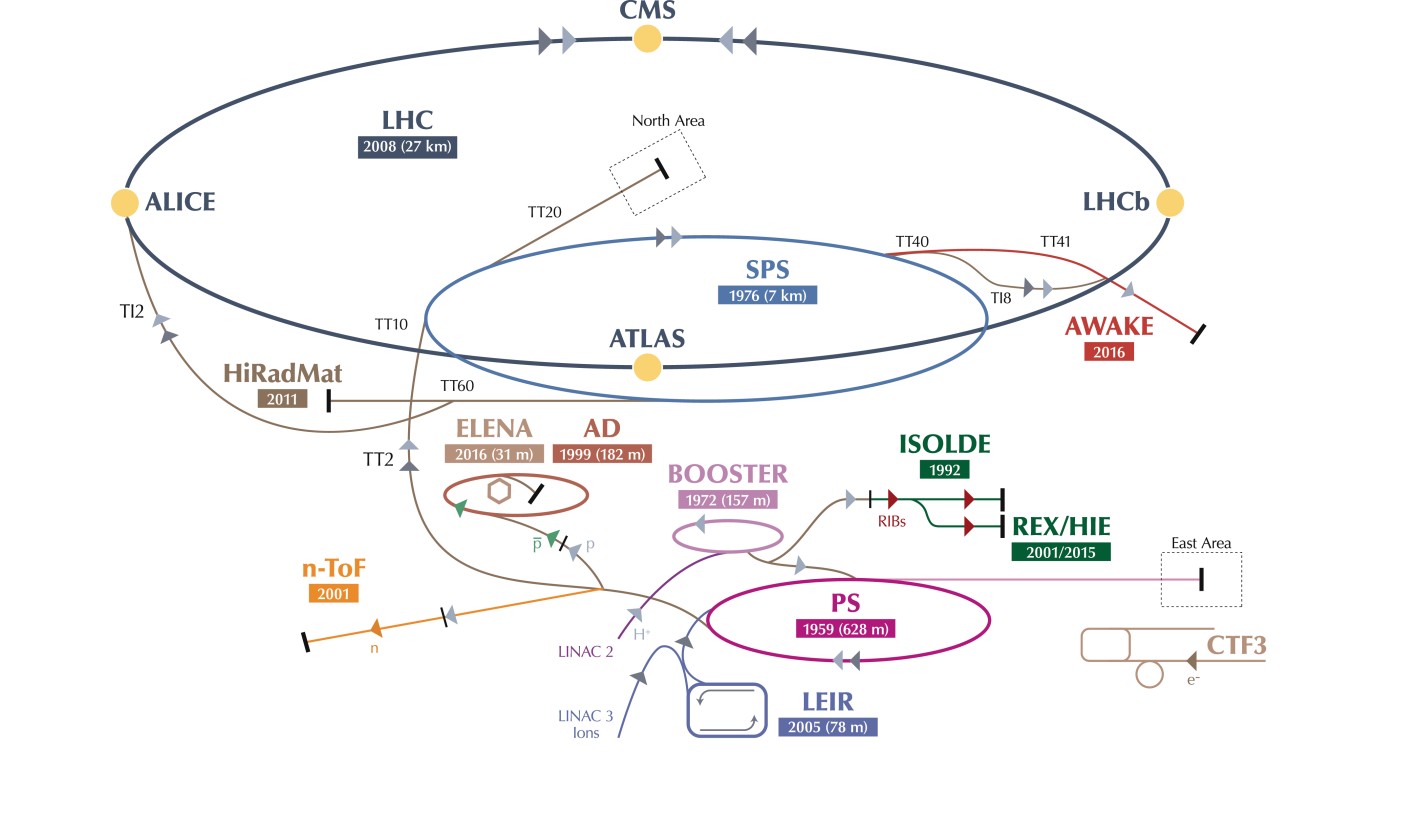
\includegraphics[width=1.\textwidth]{2_ExperimentalSetup/Figures/CCC-v2016}
 	\caption{Schematic representation of the accelerator complex at CERN~\cite{DeMelis:2197559}. The LHC (dark blue) is the last element in chain of accelerators. Protons are successively accelerated by LINAC 2, the Booster, the Proton Synchrotron (PS) and the Super Proton Synchrotron (SPS) before entering the LHC.}
 	\label{fig:LHCchain}
 \end{figure}

In \fig{fig:lhcschedule} the LHC programme is shown. the first data collisions, so-called Run 1 period, lasted from 2008 until 16 February 2013 after which  the CERN accelerator complex shut down for two years of planned maintenance and consolidation during so-called long shutdown 1 (LS1). On 23 March 2015, the new data taking period known as Run 2 started. There was a brief end of the year extended technical stop (EYETS) at the end of 2016. The main activities carried out during the EYETS were the maintenance of systems such as the cryogenics, the cooling, electrical systems, etc., the replacement of the magnet, as well as a de-cabling and cabling campaign on the SPS~\cite{MurilloQuijada:2017agx}. Run 2 will last until July 2018 when the  long shutdown 2 (LS2) will begin for 2 years. The main goal of this shutdown is the LHC injectors upgrade (LUI), but also maintenance and consolidation will be performed. Furthermore, preparations for the High Luminosity LHC (HL-LHC), which will start in 2024, will be done. More information about phase 1 upgrades during the LS1 and the EYETS in 2016 is given in \Sec{sec:Phase1}.\\ %https://home.cern/cern-people/updates/2017/01/eyets-report-so-far-so-good\
 Before the start of the LHC in 2010, the previous energy record was held by the Tevatron collider at Fermilab, colliding protons with antiprotons at \com = 1.96~\TeV.  When completely filled, the LHC nominally contains 2220 bunches in Run 2, compared to 1380 in Run 1. % (design: 2200). 
%At full intensity, it would have nearly 2800 bunches but this is limited due to a problem with SPS in 2016.
\begin{figure}[htbp]
	\centering
	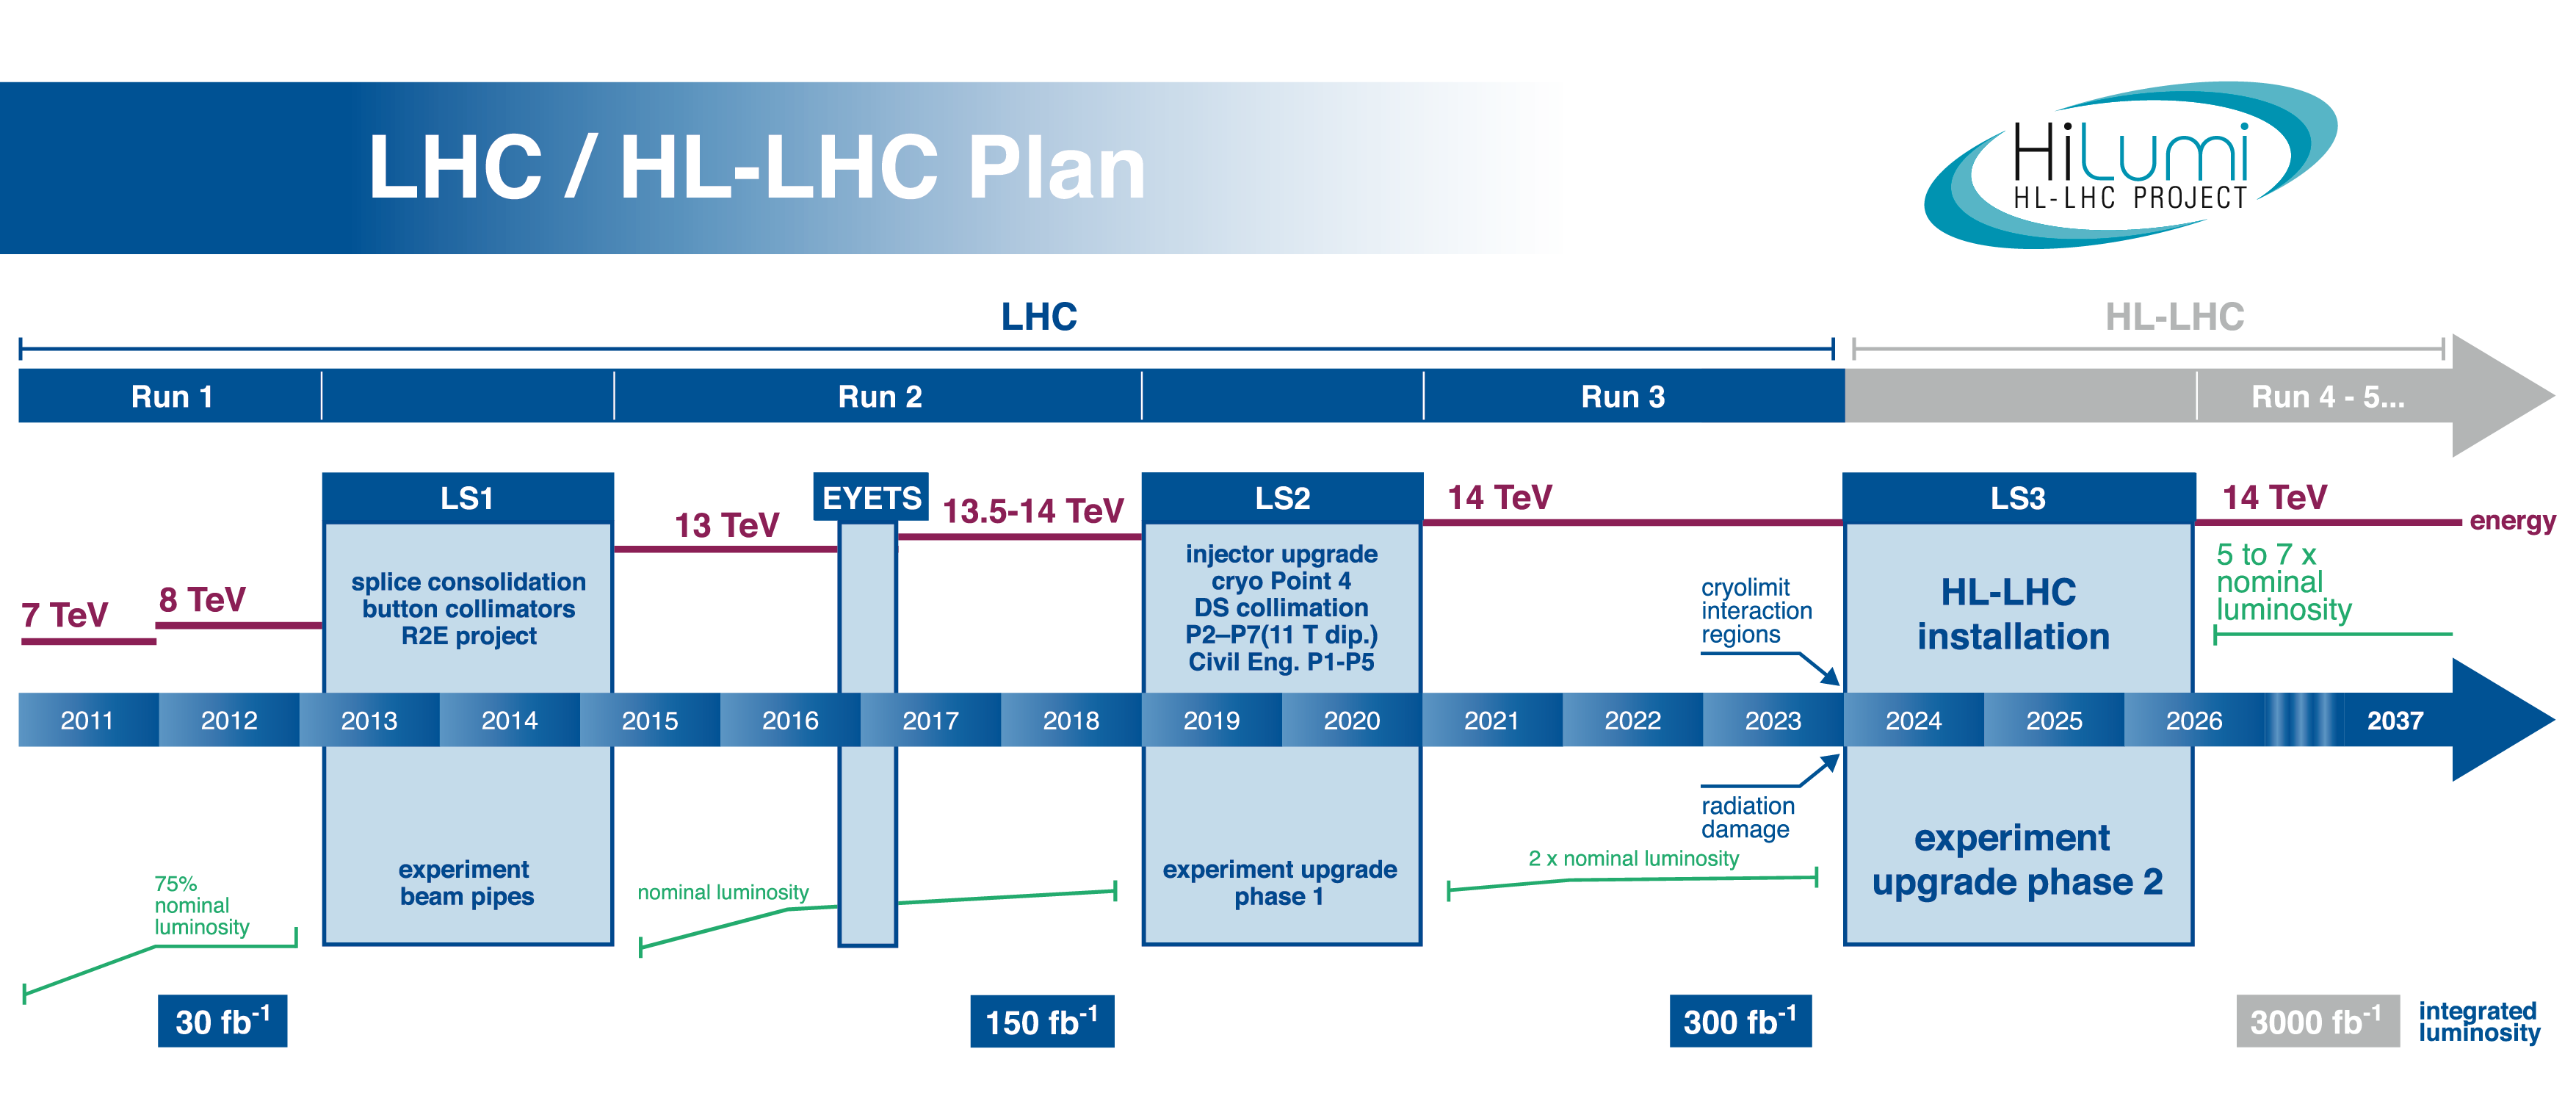
\includegraphics[width=1.\linewidth]{2_ExperimentalSetup/Figures/lhc_schedule}
	\caption{The HL-LHC timeline. Figure taken from \cite{Antonella:1975962}.}
	\label{fig:lhcschedule}
\end{figure}


Inside the LHC ring~\cite{Bruning:782076}, the protons are accelerated by the means of radio frequency cavities, while 1232 dipole magnets of approximately 15~\m\ long, each weighing 35~\tonne\, ensure the deflection of the beams.  The two proton beams circulate in opposite direction in separate pipes inside of the magnet. Through the use of a strong electric current in the coils of the magnet, magnetic fields are generated and cause the protons to bend in the required orbits. In order for the coil to become superconducting and able to produce a strong magnetic field of 8.3~\tesla, the magnet structure is surrounded by a vessel. This vessel is filled with liquid Helium making it possible to cool down the magnet to 1.9~\kelvin. In order to get more focussed and stabilised proton beams, additional higher-order multipole and corrector magnets are placed along the LHC beam line.

  

The LHC is home to seven experiments, each located at an interaction point: 
\begin{itemize}
	\item A Toroidal LHC ApparatuS (ATLAS)~\cite{Aad:2008zzm} and the Compact Muon Solenoid (CMS)~\cite{Chatrchyan:2008aa} experiments are the two general purpose detectors at the LHC. They both have a hermetic, cylindrical structure and were designed to search for new physics phenomena along with precision measurements of the Standard Model. The existence of two distinct experiments allows cross-confirmation of any discovery. 
	\item A Large Ion Collider Experiment (ALICE)~\cite{Aamodt:2008zz} and the LHC Beauty (LHCb)~\cite{Alves:2008zz} experiments are focusing on specific phenomena. ALICE studies strongly interacting matter at extreme energy densities where a quark-gluon plasma forms in heavy ion collisions (Pb-Pb or p-Pb). LHCb searches for differences between matter and antimatter with the focus on \Pbottom\ quark physics.
	\item The forward LHC (LHCf)~\cite{Bongi:2010zz} and the TOTal cross section, Elastic scattering and diffraction dissociation Measurement (TOTEM)~\cite{Anelli:2008zza} experiments are two smaller experiments that focus on head-on collisions. LHCf consists of two parts placed before and after ATLAS and studies particles created at very small angles. TOTEM is placed in the same cavern as CMS and measures the total proton-proton cross section and studies elastic and diffractive scattering.  
		\item The Monopoles and Exotics Detector At the LHC (MoEDAL)~\cite{Acharya:2014nyr} experiment is situated near LHCb and tries to find magnetic monopoles. 
\end{itemize}



 For the enhancement of the exploration of rare events and thus enhancing the number of collisions, high beam energies as well as high beam intensities are required. The luminosity~\cite{Gillies:1997001} is a measurement of the number of collisions that can be produced in a detector per square meter and per second and is the key role player in this enhancement. The LHC collisions create a number of events per second given by
\begin{equation}\label{eq:NbEv}
\centering
N_{\mathrm{event}} = L \sigma_{\mathrm{event}}, 
\end{equation}
where $\sigma_{\mathrm{event}}$ is the cross section of the process of interest and $L$ the machine  instantaneous luminosity. This luminosity depends only on the beam parameters and is for a Gaussian beam expressed as 
\begin{equation}\label{eq:Lumi}
	L = \frac{1}{4\pi}\textcolor{blue}{N_{\mathrm{b}} n_{\mathrm{b}} f_{rev}}\textcolor{red}{\frac{N_{\mathrm{b}}}{\epsilon_n }}\textcolor{darkgreen}{\left(1+\left(\frac{\theta_c \sigma_z}{2\sigma^*} \right)^2\right)^{-\frac{1}{2}}} \frac{\gamma_{\mathrm{r}}}{ \beta^*}.
\end{equation}
The number of particles per bunch is expressed by $N_{\mathrm{b}}$, while $n_{\mathrm{b}}$ is the number of bunches per beam, $f_{\mathrm{rev}}$ the revolution frequency, $\gamma_{\mathrm{r}}$ the relativistic gamma factor, $\epsilon_n$ the normalized transverse beam emittance - a quality for the confinement of the beam  , $\beta^*$ the beta function at the collision point - a measurement for the width of the beam, $\theta_c$ the angle between two beams at the interaction point, $\sigma_{\mathrm{z}}$ the mean length of one bunch, and $\sigma^*$ the mean height of one bunch. In \eq{eq:Lumi}, the blue part represents the stream of particles, the red part  the brilliance, and the green part  the geometric reduction factor due to the crossing angle at the interaction point.

The peak design luminosity for the LHC is $10^{34}\:\centi\m^{-2}\s^{-1}$, which leads to about 1 billion proton interactions per second. In 2016, the LHC was around 10\% above this design luminosity~\cite{Harriet:2212301}. The luminosity is not a constant in time since it diminishes due to collisions between the beams, and the interaction of the protons and the particle gas that is trapped in the centre of the vacuum tubes due to the magnetic field. The diffusion of the beam degrades the emittance and therefore also the luminosity. For this reason, the mean lifetime of a beam inside the LHC is around 15~\hour. The integrated luminosity - the luminosity provided in a certain time range - recorded by CMS and ATLAS over the year 2016 is given in \fig{fig:IntLumi}. In Run 2, the peak luminosity is 13-17$ \times 10^{33}\; \centi\m^{-2}\s^{-1}$ compared to 7.7$ \times 10^{33}\; \centi\m^{-2}\s^{-1}$ in Run~1. The recorded luminosity is validated for physics analysis keeping 35.9~\fbinv\ during 2016 data taking. 
% https://science.energy.gov/~/media/hep/hepap/pdf/201512/CMSRestart_Rakness_HEPAP_20151210.pdf
 \begin{figure}[htbp]
 	\centering
%	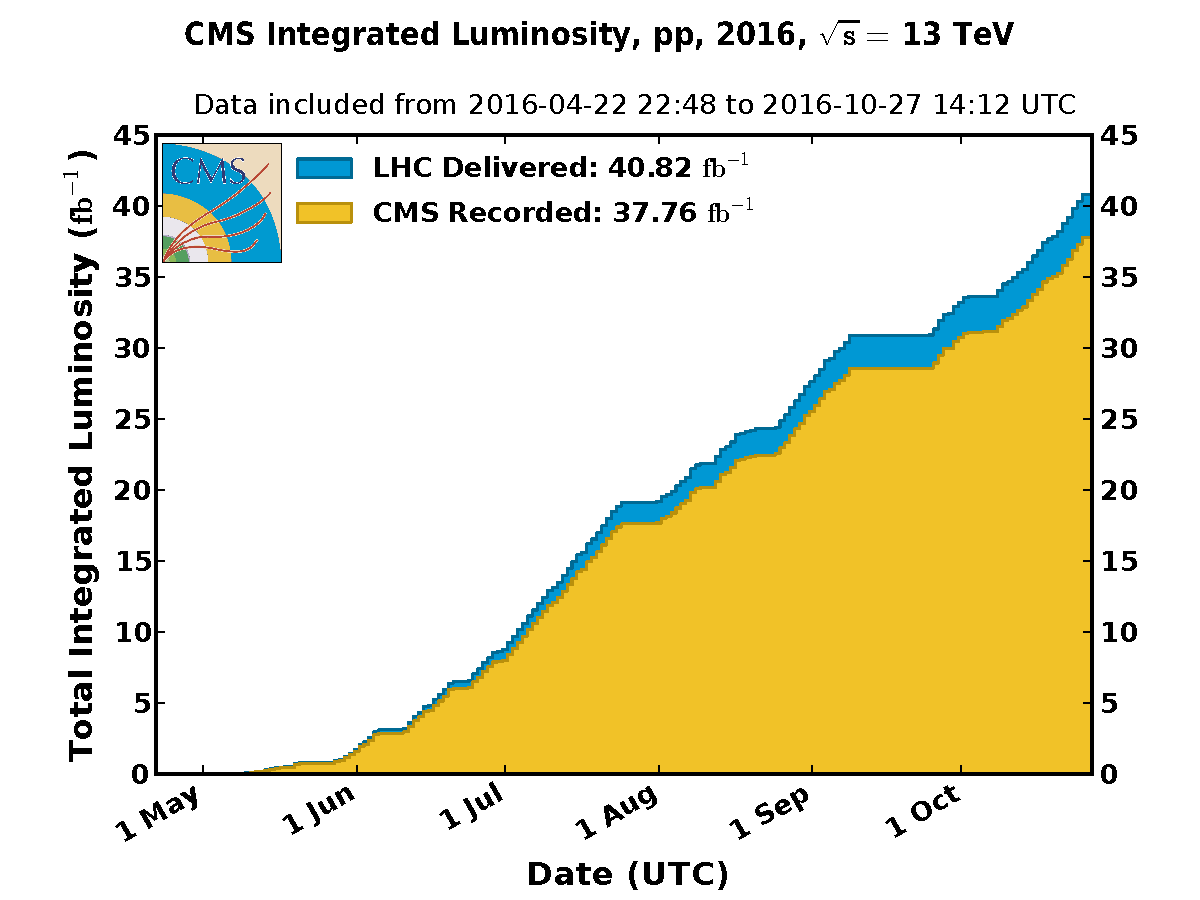
\includegraphics[width=0.7\textwidth]{2_ExperimentalSetup/Figures/int_lumi_per_day_cumulative_pp_2016.pdf}
	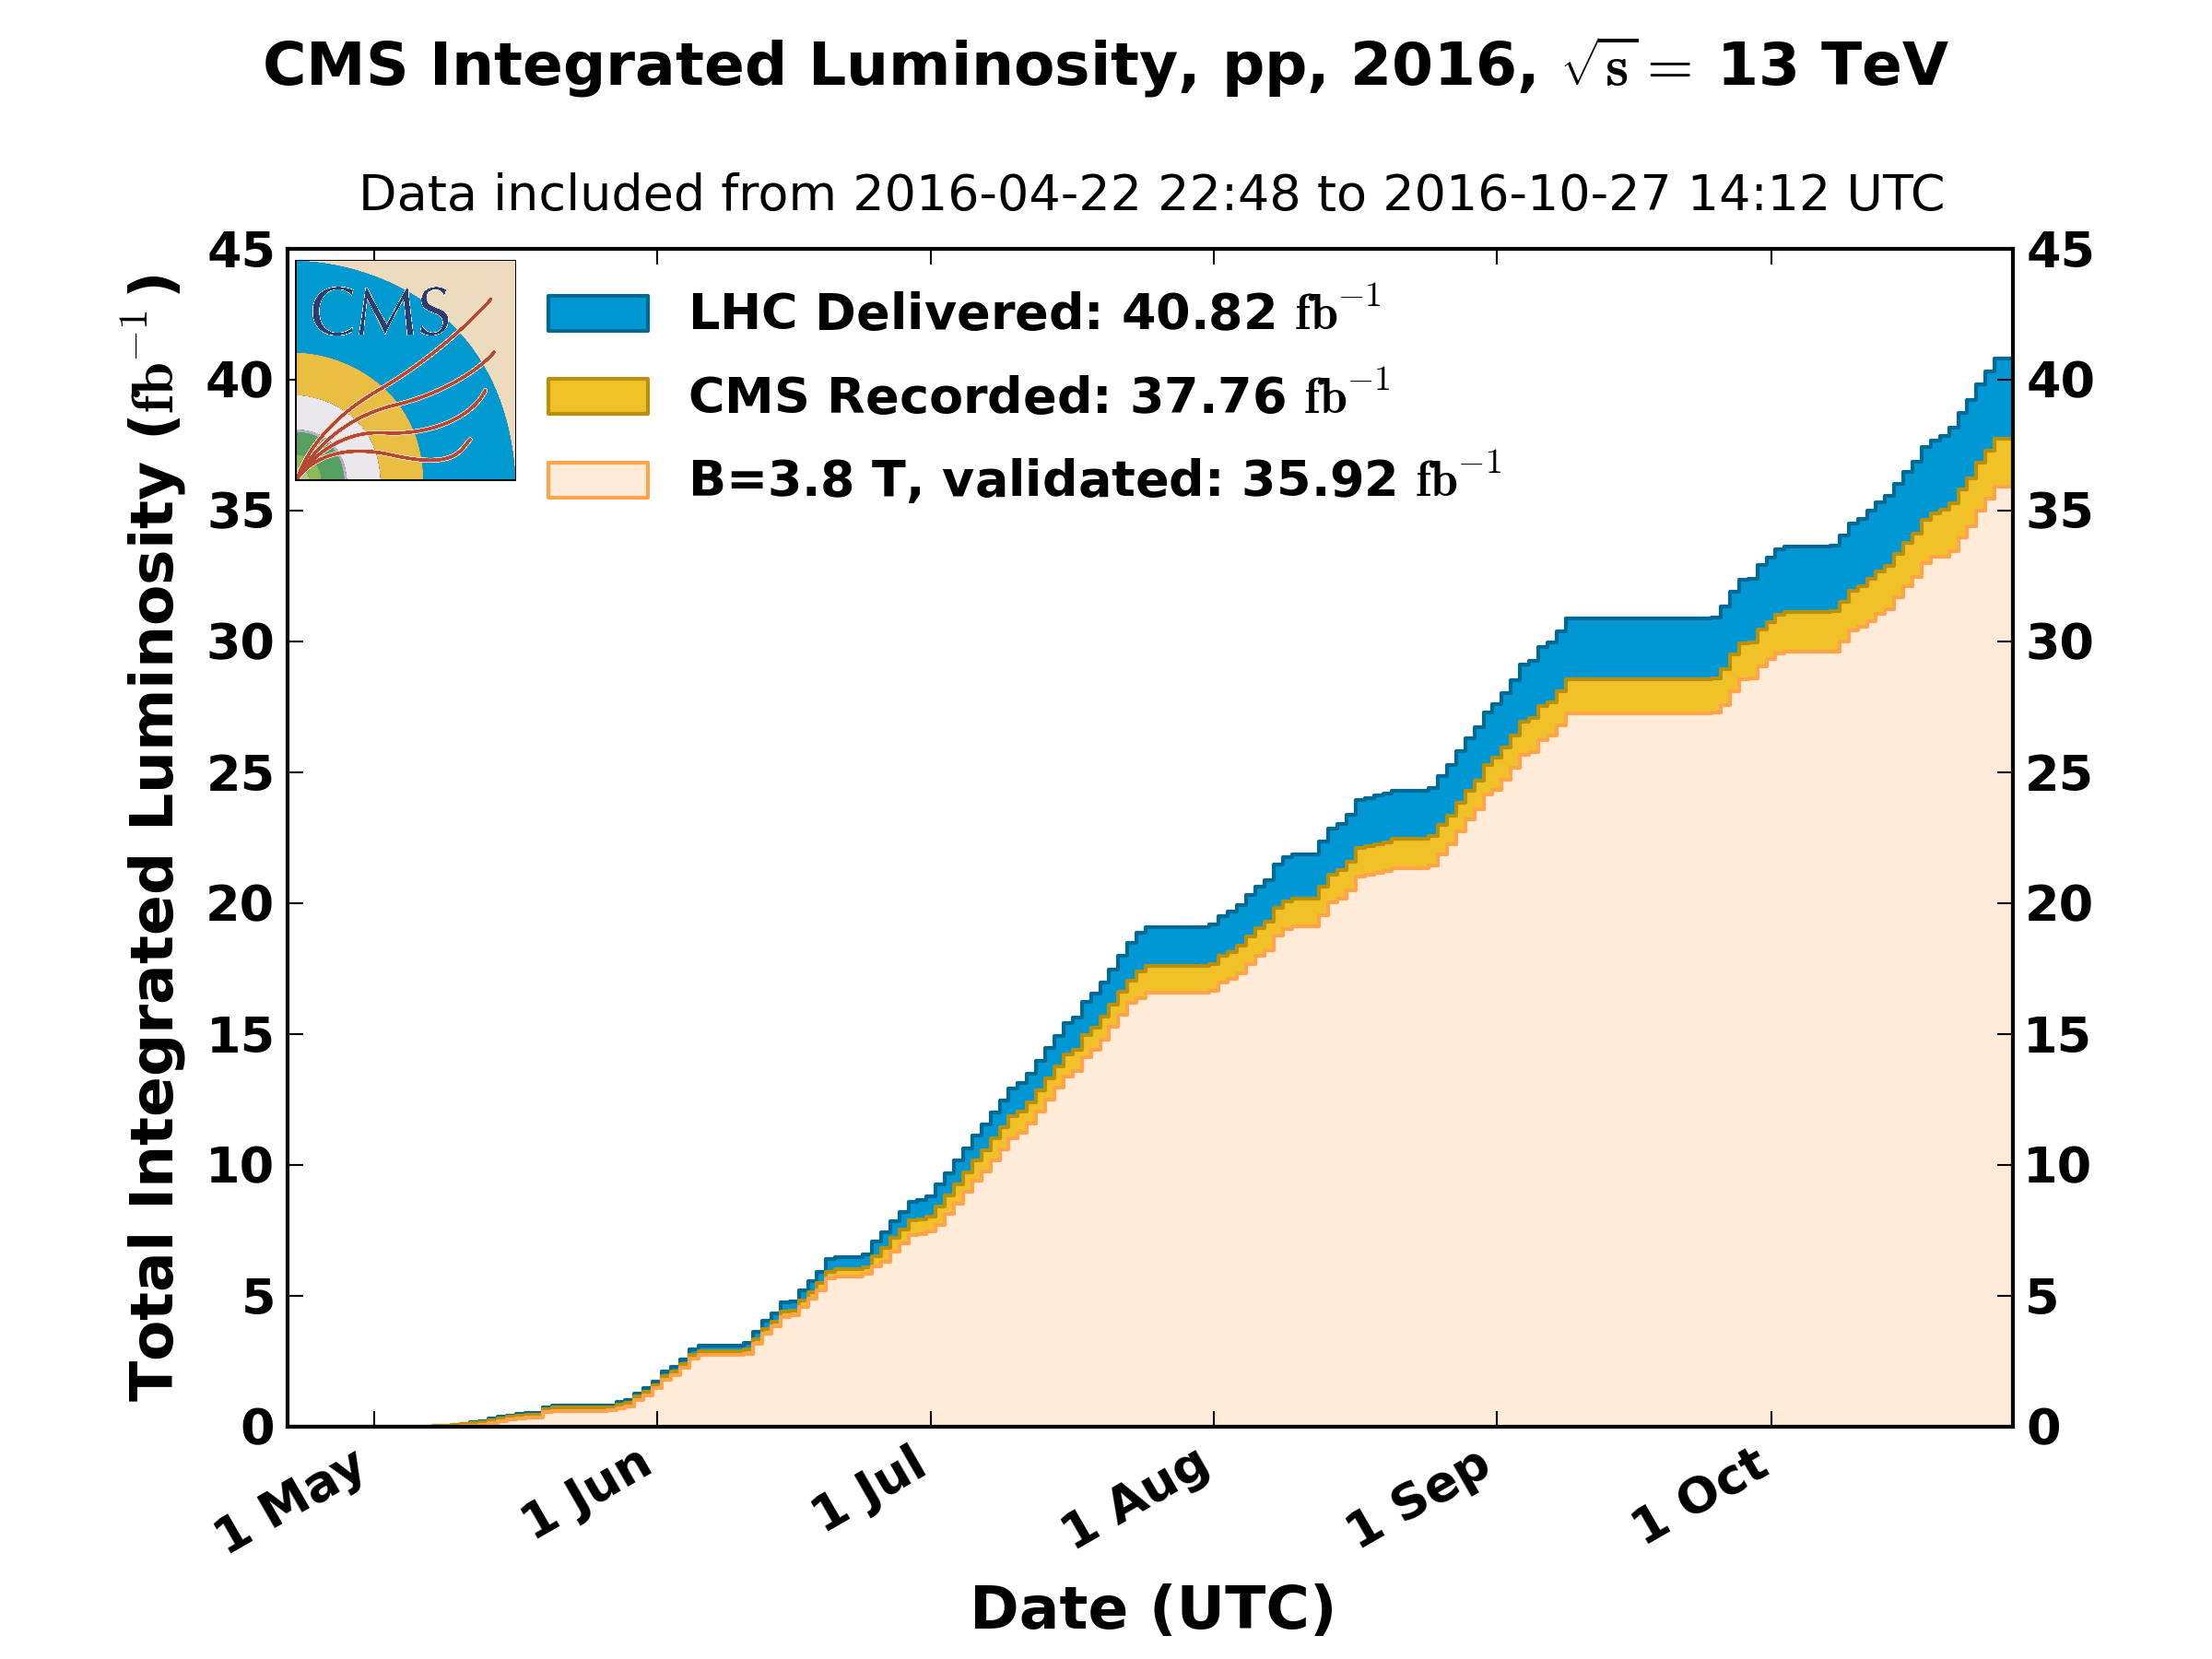
\includegraphics[width=0.7\textwidth]{2_ExperimentalSetup/Figures/int_lumi_per_day_cumulative_pp_2016_Golden_23Sep-PromEraH_Morion}
	\caption{Cumulative offline luminosity measured versus day delivered by the LHC  (blue), and recorded by CMS (orange), and certified as good for physics analysis during stable beams (light orange) during stable beams and for proton collisions at 13 TeV centre-of-mass energy in 2016.~\cite{LumiWiki}. }
	\label{fig:IntLumi}
%	(from https://twiki.cern.ch/twiki/bin/view/CMSPublic/LumiPublicResults#Online_Luminosity_AN2 )
%  https://twiki.cern.ch/twiki/bin/view/CMSPublic/DataQuality#2016_Proton_Proton_Collisions
\end{figure}
 
Multiple proton-proton interactions can occur during one  bunch crossing, referred to as \pu. On average, the number of \pu\ events is proportional to the luminosity times the total inelastic proton-proton cross section. In 2016,  an average of about 27 of \pu\ interactions has been observed in 13 \TeV\ proton collisions at the interaction point of CMS. For 2012, this number was about 21 \pu\ interactions for 8 \TeV\ collisions.



%CMS collaboration http://cds.cern.ch/record/2195940?ln=en map
